%!TEX root = ../report.tex

\chapter{Evaluation}
\label{chap:evaluation}
\section{Hardware}
\label{gpu}
All the computational tasks has been carried out in the cluster computation environment (Platform for Scientific Computing at Bonn-Rhein-Sieg University). For CNN training and evaluation GPU nodes were used which has the following specifications:
\begin{itemize}
 \item Barebone Dell PowerEdge R740
 \item 2 Intel Xeon Gold 6130 at 2.1 GHz with in total 64 hardware threads 
 \item 192 GB DDR4-2466 memory
 \item 480 GB SSD
 \item Nvidia Tesla V100 with 16 GB memory
 \item 100 Gb/s Intel Omni-Path adapter Intel 100HFA016LS
\end{itemize}

The GPU nodes used CUDA \cite{cuda} driver version 9.2 for accelerated computing. For interactive computing node wr14 with GPU Nvidia, Tesla K80 has been used. More details can be found here \cite{cluster}.

\section{Software}
The code for the evaluation are written in Python (version 3.6.6) \cite{python}. For the deep learning tasks, Keras (version 2.2.2) \cite{chollet2015keras} with TensorFlow (version 1.10.0) \cite{tensorflow} as backend is used. For train/test
data split and computing area under ROC curve scikit-learn (version 0.20.0) \cite{sklearn} was used.

\section{Evaluation Metric And Process}
This section contains details of how all three networks are optimized and evaluated. After a brief description of how the Area under ROC is obtained, the description of the grid search process for hyperparameter optimization is presented.
\subsection{Receiver Operating Characteristic}
In Wikipedia \cite{wikiroc}, the definition of Receiver operating characteristic (ROC) curve, is as follows, ``ROC curve is a graphical plot that illustrates the diagnostic ability of a binary classifier system as its discrimination threshold is varied.'' 
To compute the ROC curve the true positive rate (TPR) and the false positive rate (FPR) are computed for a binary-classifier, for all possible values of thresholds. Then by plotting the TPR against FPR, the ROC curve for the classifier is obtained.

The metric AUC is just the area under the ROC curve. AUC is equal to the probability that a classifier will predict a higher score for a random positive test case over a random negative test case \cite{wikiroc}. Where positive is assumed to be of higher rank.
AUC as a metric is different than accuracy. Accuracy can be computed based on a fixed threshold on the prediction score. AUC, on the other hand, represents how classifier performs over all possible values of the threshold. Since AUC is not a function 
of a fixed threshold, it can be seen as a more comprehensive measure than just accuracy, though that is fairly situational.
The dataset used here for training and testing is both balanced with positive and negative samples. So selecting AUC as the metric for performance evaluation of the convolutional networks is a sound approach. 
AUC value of 0.5 can be compared to the area under a vertical line connecting (0,0) and (1,1), in the ROC curve. A random chance falls under this line and has less than equals to 0.5 AUC. A classifier with AUC values higher than 0.8 AUC can be considered very good, while 1.0 is the best possible AUC.

\subsection{Hyperparameter Optimization}
Hyperparameter optimization is a very common challenge in a machine-learning problem. The optimization process starts with the identification of all the hyperparameters which influence the learning process. Then, optimal values for those parameters
need to be searched, which will maximize the learning capacity of the network. Learning the training data is important but the network should also generalize well. There are different methods for hyperparameter optimization. The preferred choice
of method is automatic hyperparameter optimization with Hyperas \ref{chap:hyperas}. But two main challenges forced further progress in that direction. Firstly, the computation environment available \ref{gpu} has a time limit of only 
3 days. For a thorough automated hyperparameter optimization, depending on the number of total parameters and the fineness of search space, 3 days is not enough time to converge to an optimal solution. For DenseNet architectures, there are a lot of hyperparameters
which were to be optimized. By dividing the search space into smaller and more focused search space this challenge has been addressed. But, the hyperparameter search for DenseNet-Siamese failed repeatedly after few runs due to GPU 
memory issue, (\code{std::bad\_alloc}). After a few weeks of trials and contacting responsible persons from Cluster administration and Hyperas both, this problem did not get resolved. Since the GPU has a memory of 16 GB in the cluster, the issue is probably with the efficiency of the garbage collection and memory usage of the framework. DenseNet can consume a lot of memory and the DenseNet-Siamese is the biggest network that needs to be evaluated in the scope of this thesis. But this memory issue
did not occur for the manual grid search. Hence it became the choice of method for hyperparameter optimization.

%\begin{figure}[ht]
%\centering
%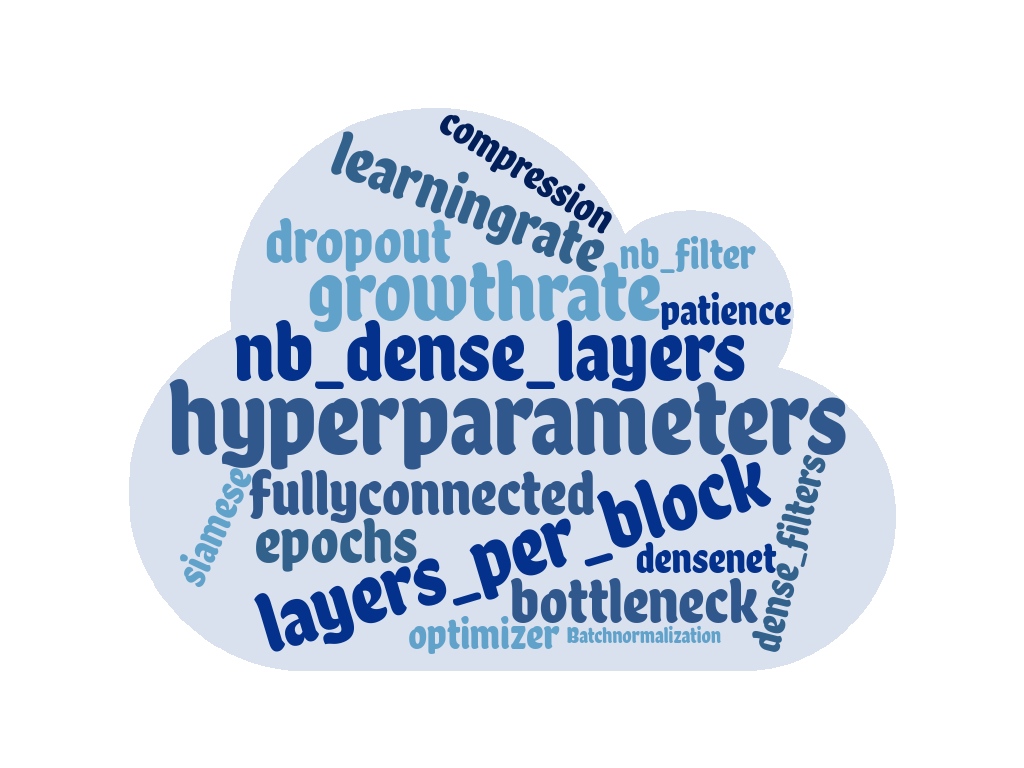
\includegraphics[width=0.5\textwidth]{images/densenet/wordcloud_hyperparameters.png}
%\caption{\label{fig:wordcloud_hp}Hyper parameters word cloud.}
%\end{figure}

\subsection{Grid Search Method}
For the manual grid search the search space manually defined and supplied to the evaluation script externally. An example of search space is displayed in table \ref{table:grid_example}.

\begin{table}
\centering
    \begin{tabular}{|c c c c c|} 
      \hline\hline
      Epochs & Optimizer & Batch size & Dropout & Use batch norm\\[0.5ex] 
      \hline
      5 & adam & 64 & 0.4 & True \\  
      \hline
      5 & adam & 64 & 0.4 & False \\ 
      %\hline
      %5 & adam & 64 & 0.7 & False \\ 
      %\hline
      %8 & rmsprop & 64 & 0.4 & True\\ 
      \hline \hline
    \end{tabular}
  \caption{Custom grid search space example.}
  \label{table:grid_example}
\end{table}

The example displayed in table \ref{table:grid_example} presents how the search space is predefined to evaluate different cases, here the effect of using batch normalization can be investigated by comparing the results of two test cases.
The predefined search grid passed as input to the actual code and the configurations are applied one by one and evaluated sequentially. In \ref{table:grid_example} the value for 'use batch norm' is set to 'True', after parsing this test case the use of batch normalization layer is activated for the network, where applicable. 

For the evaluation the epochs are set after multiple testings in order to ensure, the networks do not get overtrained and good generalization is obtained. Also if the network is undertrained, then 
it will not generalize well. Setting the epochs effectively were one of the big challenge of this work, because in some cases the networks gets overtrained after 4-5 epochs. In general Siamese network trains very fast.

\subsection{Training Process}
The train data has been divided into the train and validation data randomly using Sklearn train test data split \cite{sklearnsplit} in \textbf{8:2 ratio}. This is done using \textbf{fixed seed} to ensure the validation and train cases are the same for all the evaluations across all three methods. It is important to clarify that the role of the validation data in Keras is different than classical training methods. In Keras the validation data is \textbf{not} used to update the weights. Instead, the validation dataset can be used to monitor the network performance in terms of validation accuracy and validation loss. Using callback functions such as \code{EarlyStopping} and \code{ReduceLROnPlateu} \cite{kerascallbacks} the network validation performance can be monitored after each epoch of training.
By configuring the callbacks properly (parameter: 'Early stop patience') the training can be stopped if the validation accuracy or loss does not improve after a number of epochs.
Similarly, if the validation performance does not improve after some epochs the learning rate can be reduced by a previously determined factor (by configuring \code{ReduceLROnPlateu}) to come out of the local minima. The patience values are set after some manual trials for different network settings. the following is an example of how the callbacks can be configured in Keras \cite{kerascallbacks}. \code{ModelCheckpoint} is a callback which saves the best weight of the network 
after each epoch, if a certain condition is met, e.g. validation loss is improved.\\

\begin{lstlisting}
#Early stopping
es = EarlyStopping(monitor='val_acc', patience=es_patience,verbose=1)
#Model check point
checkpointer = ModelCheckpoint(filepath=weight_file, verbose=2, save_best_only=True) 
#Learning rate reducer on plateu
lr_reducer = ReduceLROnPlateau(monitor='val_loss', factor=np.sqrt(0.1), cooldown=0, patience=lr_patience, min_lr=0.5e-6,verbose=1)
\end{lstlisting}

